\section{Exponentielle Algorithmen}
\paragraph{Beispiel:}
Traveling Salesman Problem
\begin{figure}[H]
	\centering
	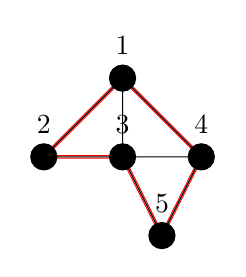
\begin{tikzpicture}
	\draw[draw=red, fill=none, double distance=0.5] (0,1)--(-1,0)--(0,0)--(.5,-1)--(1,0)--(0,1);
	\draw[draw] (0,1) node[draw, fill, circle, label=1]{}
		--(-1,0) node[draw, fill, circle, label=2]{}
		--(0,0) node[draw, fill, circle, label=3]{}
		--(1,0) node[draw, fill, circle, label = 4]{}
		--(.5,-1) node[draw, fill, circle, label = 5]{}
		--(0,0) --(0,1)--(1,0);
	\end{tikzpicture}
\end{figure}
\begin{itemize}
	\item Gegeben Graph $G=(\overset{=\{1,\ldots,n \}}{V},E)$, Kantenkosten $c:E\rightarrow \mathbb{R}$
	\item Gesucht: Zyklus, der jeden Knoten genau ein Mal besucht und minimale Kosten hat.
\end{itemize}
\subsection{Trivialer Algorithmus}
Iteriere über alle Permutationen der Knoten, berchne jeweils die Kosten der Tour und speichere die billigste.
\subsubsection{Laufzeit}
\[ O(n!\cdot m) \]
Für $f:\mathbb{N}\rightarrow\mathbb{N}$ definieren wir:
\[ O^*(f) : \{ g:\mathbb{N}\rightarrow\mathbb{N} | g(n) \leq f(n)\cdot \text{poly}(m) \} \]
für ein Polynom $p$\\
\paragraph{Also:}
Algorithmus hat eine Laufzeit von $O^*(n!)$\\
\paragraph{Ziel:}
Algorithmus für TSP der bzgl. der $O^*$-Notation schneller ist. (einen Algorithmus mit Laufzeit $O^*(2^m)$)\\
Für alle $\{1\}\subseteq S \subseteq V$ und alle $v\in S$ berechnen wir:\\
$O(S,v)=$ Kürzester Pfad, der jeden Knoten in S genau ein Mal besucht und in $v$ endet.\\
Die Länge der TSP-Tour ist dann
\[ \underset{2\leq i \leq n}{\min}O(V,I) + c(i,1) \]
\begin{figure}[H]
	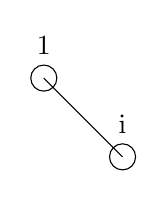
\begin{tikzpicture}
	\draw (1,1) node[draw, circle, label=1]{}
	--(2,0) node[draw, circle, label=i]{};
	%curly pfad von i nach 1 mit zwischen Stopps und beschriftung O(V,i) 
	\end{tikzpicture}
\end{figure}
$O(S,i)$ können wir wie folgt berechnen:
\[ O({1},1) = 0 \]
\[ \underset{2^n \text{Werte}}{\underbrace{O(S,i)}} = \underset{j\in S\setminus\{i\} }{O(S\setminus\{1\}, j  ) + c(j,i)} \]
%Bild mit großem S links und curly Pfad von 1 über zwischenstopps nach j und dann direkt nach i
\subsection{Laufzeit}
\[ O^*(2^n) \]
\paragraph{Beispiel}
\section{Vertex-Cover (VC)-Problem}
\begin{figure}[H]
	\centering
	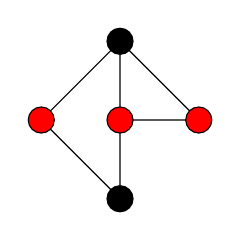
\begin{tikzpicture}
	\draw (0,1) node[draw, fill, circle]{} 
	-- (-1,0) node[draw, fill={red}, circle] {}
	-- (0,-1) node[draw, fill, circle] {}
	-- (0,0) node[draw, fill={red}, circle] {}
	-- (1,0) node[draw, fill={red}, circle] {}
	-- (0,1) --(0,0);
	\end{tikzpicture}
\end{figure}
\begin{itemize}
	\item Gegeben: Graph $G=(V,E)$
	\item VC: Teilmenge $U\subseteq V$, so dass $e\cap U \neq \emptyset$ für alle $e\in E$
	\item Gesucht: VC minimaler Kardinalität
\end{itemize}
\subsection{Trivialer Algorithmus}
Probiere alle Teilmengen $U\subset V$ aus
\subsection{Laufzeit}
$O^*(2^n)$
\section{Branching-Algorithmus für VC}
Wir wählen $v\in V$ und machen die Fallunterscheidung $u\in U$ und $u \notin U$
\begin{description}
	\item[\textbullet $u\in U$:] Alle Kanten adjazent zu $u$ sind damit überdeckt und man löst rekursiv das Problem ohne $v$ und dessen adjazenten Kanten
	\item[\textbullet $u\in V$:] Alle zu $v$ inzidenten Knoten müssen zu $U$ hinzugefügt werden und nun löst ma das Problem auf dem Graphen, in dem alle diese Knoten und deren adjazenten Kanten gelöscht werden
\end{description}
\subsection{Pseudocode}
\begin{lstlisting}
finde\_VC(G=(V,E))
	- entferne alle Knoten vom Grad 0
	- Sei $u\in V$
	- $S_1$ = find_VC$ (G[ V\setminus \{ u \}]) \cup \{u\} $
	- $S_2$ = find_VC$ (G[ V\setminus \{ u \} \setminus \underset{\text{Nachbarn von n}}{\underbrace{N[u]}} ]) \cup N[u] $
	- return kleineres von $S_1$ und $S_2$  
\end{lstlisting}
\subsubsection{Laufzeit}
Da wir "`nur"' bzgl. der $O^*$-Notation analysieren, analysieren wir $T(n):$ maximale mögliche Anzahl von Teilproblemen bei einem Graph mit $n$ Knoten\\
Rekursionsgleichung für $T(n)$: (Annahme $T$ wächst monoton)
\begin{align*}
T(n) \leq \begin{cases}
T(n-1) + T(n-2)& \text{für} n\geq 2\\
1 & \text{für} n \leq 1
\end{cases}
\end{align*}
Fibonacci-Zahlen, also $T(n) \leq \left( \frac{1 + \sqrt{5}}{2} \right)^n \approx 1,618^n$
\subsubsection{Laufzeit}
\[ O^*\left( \frac{1+\sqrt{5}}{2} \right)^n \]
\subsection{Verbesserung}
Statt $c\in V$ beliebig zu wählen, wähle $v$ mit maximalem Grad\\
Zuvor entfernen wir nicht nur die Knoten com Grad 0, sondern auch die vom Grad 1 mit folgender Überlegung:
\begin{figure}[H]
	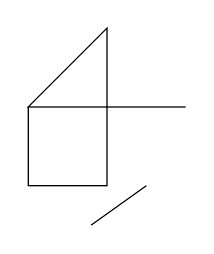
\begin{tikzpicture}
	\draw (-1,1)--(-1,0)--(0,0)--(0,2)--(-1,1)--(1,1);
	\draw (-.2,-.5)--(.5,0);
	\end{tikzpicture}
\end{figure}
\begin{itemize}
	\item Hat ein Knoten Grad 1, so nimm den anderen Endpunkt in $U$ auf und vereinfache den Graphen\\
	$\rightsquigarrow$ nun haben alle Knoten mindestens Grad 2
	\item Haben alle Knoten Grad 2, so haben wir eine Menge von Zyklen und knönnen das VC-Problem direkt lösen\\
	$\rightsquigarrow$ Wir können davon ausgehen, dass es mindestens einen Knoten vom Grad $\geq$ 3 gibt
\end{itemize}
\begin{figure}[H]
	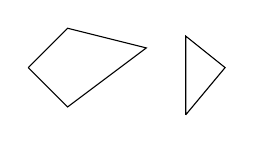
\begin{tikzpicture}
	\draw (-1,.5)--(-.5,0)--(.5,.75)--(-.5,1)--(-1,.5);
	\draw (1,-.1)--(1.5,.5)--(1,.9)--(1,-.1);
	\end{tikzpicture}
\end{figure}
Verbesserte Abschätzung für die Anzahl $T$ der Teilprobleme
\[ T(n) \leq T(n-1) + T(n-4) \in O^*(1,41^n)  \]
\section{Laufzeitanalyse vom Branching-Programm in $O^*$-Notation}
Wir wählen Rekursionsgleichung der Form:
\begin{align*}
T(n) \leq \begin{cases}
T(n-d_1) + T(n-d_2) + \ldots + T(n-d_p)& \text{für} n\geq d\\
1 & \text{für} n \leq d
\end{cases}
\end{align*}
in $O^*$-Notation abschätzen, wobei $d=\max(d_1,d_2,\ldots,d_p)$\\
Wir wollen ein möglichste kleines $\lambda \geq 0$ haben, so dass $T(n) \leq \lambda^n$\\
Wir müssen $\lambda$ so wählen, dass
\[ \lambda^n \geq \lambda^{n-d_1} + \lambda^{n-d_2} + \ldots + \lambda^{n-d_p} \]
(dann können wir mit obiger Rekursionsgleichung leicht per Induktion beweisen)
\[ T(n) \leq \delta^n \]
Umschreiben:
\[ \lambda^d \geq \lambda^{d-d_1} + \lambda^{d-d_2} + \ldots + \lambda^{d-d_p} \]
\[ \lambda^d - \lambda^{d-d_1} - \lambda^{d-d_2} - \ldots - \lambda^{d-d_p} \geq 0 \]
$P$ ist ein Polynom vom Grad $d$ und $P(0) < 0$ (solange $p>1$) und $p$ hat genau eine positive Nullstelle.\\
Diese muss man nun bestimmen und hat dann die Rekursionsgleichung gelöst.\\
Zahlenbeispiel: $T8N) \leq T(n-d_1) + T(n-d_2)$\\
\begin{tabular}{l|cccc}
	 &$1$&$2$&$3$& \\\hline
	$1$&$2$&$1,618$&$1,46$&$\cdots$ \\
	$2$& &$1,41$&$1,32$&$\cdots$\\
	$3$& & &$1,25$&$\cdots$\\
	   & & &$\vdots$&
\end{tabular}
\section{Parametrische Algorithmen aus den Klassen FPT und XP}
\begin{itemize}
	\item Wir wollen Algorithmen für NP-schwere Probleme herleiten
	\item Oft kennt man eine "`Eigenschaft"' der zu lösenden Instanzen und hofft, dass diese die Fragestellung "`einfacher"' macht
	\item Lässt sich die Eingenschaft in einer Zahl beschreiben, nenn man das Problem ein Parametrisches Problem
\end{itemize}
\paragraph{Beispiel}
Vertex-Cover mit zusätzlicher Annahme "`es existiert ein kleines Cover"'. Sei $k$ die Größe des minimalen VC. Versuche Algorithmus zu finden, der effizient ist, falls $k$ "`klein"'. (XP Algorithmus)
\subsubsection{trivialer Algorithmus}
Zähle nur Teilmengen bis zur Größe $k$ auf $\rightsquigarrow$ Laufzeit $O(n^k)$\\
Geht es besser?\\
\begin{itemize}
	\item Entferne alle Knoten vom Grad 0 und 1, wie oben
	\item Füge jeden Knoten mit Grad $\geq k+1$ zu VC hinzu (da sonst die Nachbarschaft im VC wäre und damit zu groß)
	\item Iterire
\end{itemize}
\begin{figure}[H]
	
\begin{tikzpicture}
	\draw (0,0) node[fill, circle](A){} -- (.75,.75)
	(A) --(-.75,.75)
	(A) -- (-.75,-.75)
	(A) -- (.75,-.75)
	(A) -- (0,-1); 
	\end{tikzpicture}
\end{figure}
Am Ende hat jeder Knoten einen Grad zwischen 2 und $k$.\\
\begin{figure}[H]
	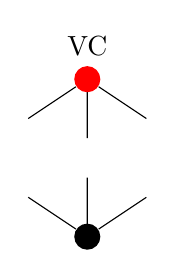
\begin{tikzpicture}
	\draw (0,1) node[fill=red, circle, label={VC}](A){} -- (0,.25)
	(A) --(-.75,.5)
	(A) -- (.75,.5);
	\draw (0,-1) node[fill, circle](B){} -- (0,-.25)
	(B) --(-.75,-.5)
	(B) -- (.75,-.5); 
	\end{tikzpicture}
	\end{figure}
Hat der Graph nun mehr als $k^2$ Knoten, so gib es kein VC mit der Kardinalität $\leq k$\\
$\rightsquigarrow$ Also kann der Graph nur $k^2$ Knoten haben.\\
Auf diesem Restgraph benutzen wir nun den Branching-Algorithmus und erzielen eine Laufzeit von $O(\underset{\text{Vereinfachen des Graphen}}{\underbrace{\text{poly}(m)}} + \left( k^2 \right)^{1,4} )$ (FPT)
\subsection{Definition}
Parametrisches Problem $L \subseteq \Sigma^* \times \mathbb{N}$ für eine Instanz $(x,t) (x \in \Sigma^*, k\in \mathbb{N} )$ heißt $x$ die Eigenschaft, $n-|x|$ die Länge der Eingabe der Parameter
\begin{itemize}
	\item Ein parametrisches Problem $L$ heißt fixed-parameter-tractable (FPT) wenn es ein en Algorithmus für $L$ gibt mit Laufzeit $f(k)\cdot m^2$ für $c\in \mathbb{N}$ und $f$ berechenbare Funktion
	\item Ein Problem heißt in XP, wenn es für jedes feste $k \in \mathbb{N}$ einen polynomischen Algorithmus für den alle Instanzen mit Parameter $k$ gibt. (Laufzeit ist immer $O(n^{f(k)})$
\end{itemize}